\subsection{Wyniki - sing-around}
\label{sec:53f}

Sekcja zawiera wyniki symulacji efektu sing-around dla sygnału chirp przedstawionego na rysunku \ref{fig:chirp}. Rysunek \ref{fig:fchirp} przedstawia widmo amplitudowe badanego sygnału. Krzywe dyspersji wykorzystane w symulacji są przedstawione w na rysunku \ref{fig:wykres4}, a za krzywe wzbudzalności posłużyły testowe krzywe eksponencjalne ukazane na rysunku \ref{fig:singExc}.

\begin{figure}[h]
\centering
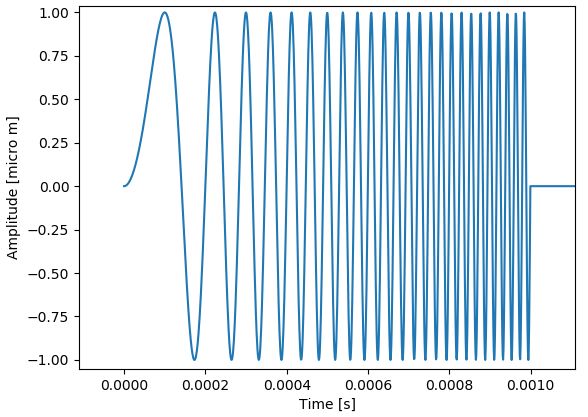
\includegraphics[width=10cm]{Zdjecia/5/chirp1}
\caption{Sygnał chirp}
\label{fig:chirp}
\end{figure}

\begin{figure}[h]
\centering
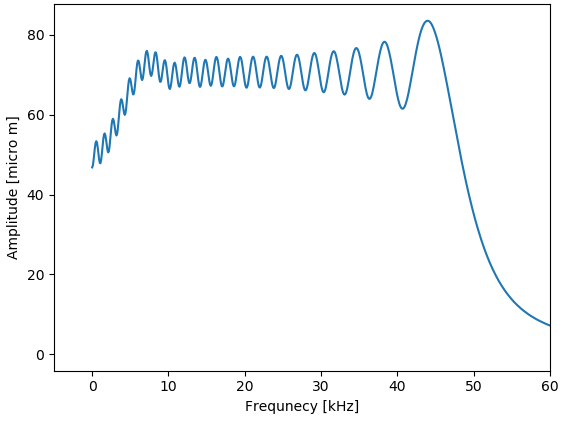
\includegraphics[width=10cm]{Zdjecia/5/chirp_widmo}
\caption{Widmo sygnał chirp}
\label{fig:fchirp}
\end{figure}

\begin{figure}[h]
\centering
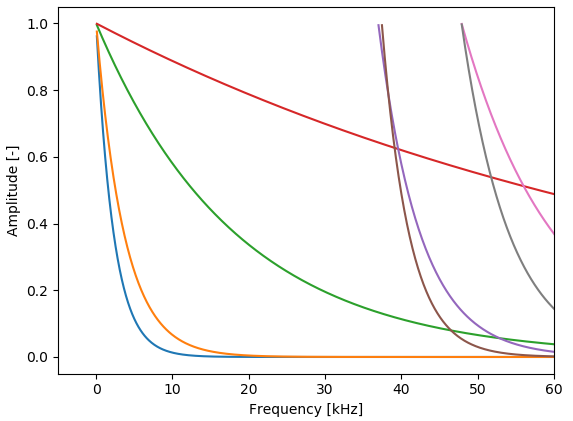
\includegraphics[width=10cm]{Zdjecia/5/krzywe_wzbudzalnosci}
\caption{Krzywe wykorzystane w roli krzywych wzbudzalności}
\label{fig:singExc}
\end{figure}

Rysunku \ref{fig:1prop} i \ref{fig:8prop} przedstawiają wyniki symulacji po 1 przejściu i po 8 kolejnych przejściach fali na długości 2 metrów.

\begin{figure}[h]
\centering
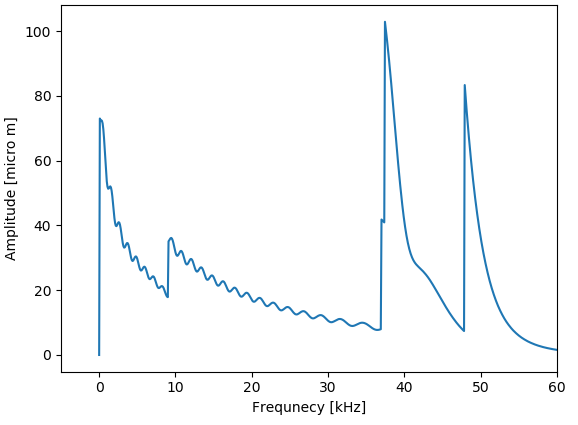
\includegraphics[width=10cm]{Zdjecia/5/1}
\caption{Widmo sygnału po jednym przejściu fali}
\label{fig:1prop}
\end{figure}

\begin{figure}[h]
\centering
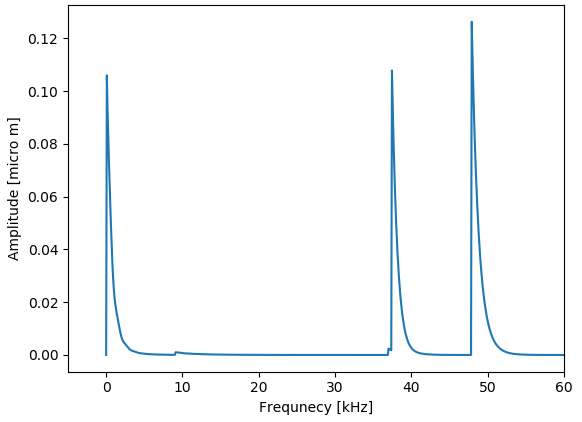
\includegraphics[width=10cm]{Zdjecia/5/8}
\caption{Widmo sygnału po ośmiu przejściach fali}
\label{fig:8prop}
\end{figure}

Przesunięcia fazowe sygnału nie powodują zmiany jego widma amplitudowego. Uwzględnienie krzywych wzbudzalności powoduje natomiast ukazanie się częstotliwości rezonansowych obiektu. Kolejne przejścia powodują, że częstotliwości rezonansowe są coraz bardziej uwidocznione.

Wykrywanie tego typu częstotliwości w sygnale ma duże zatosowanie w badaniu stanu konstrukcji. Problemem może się okazać dostosowanie czasu, w którym występują interesujące nas częstotliwości. Efekt dyspersji powoduje, że składowe o różnych częstotliwościach poruszają się z różnymi prędkościami, a co za tym idzie mogą się nakładać raz wzmacniając, a raz wygaszając.


